\section{Calcolare il campo elettrostatico di una distribuzione
    	lineare ed uniforme di carica elettrica mediante il teorema di
    	Gauss.}
Per distribuzione lineare e uniforme di carica si intende una distribuzione di cariche su un filo nel piano $xyz$ dove vi \`e una densit\'a lineare di carica $\lambda$ costante per tutto il filo.
Si noti che :
$$ \left[\lambda\right] =  \left[\frac{Q}{m}\right] $$
   
Secondo il teorema di Gauss per il campo elettrico, vale quanto segue:
\begin{displaymath}
    \Phi_S\left(\vec{E}\right) = \oint_{S}{\vec{E} \cdot \hat{n}} = \frac{\sum{Q_{interne}}}{\varepsilon_0}
\end{displaymath}
    
Per calcolare il flusso del campo elettrico su tale distribuzione occorre quindi scegliere una opportuna superficie chiusa, per esempio un cilindro di altezza $h$ e raggio $r$ avente il centro delle sue basi sulla distribuzione.	
    
\begin{center}
	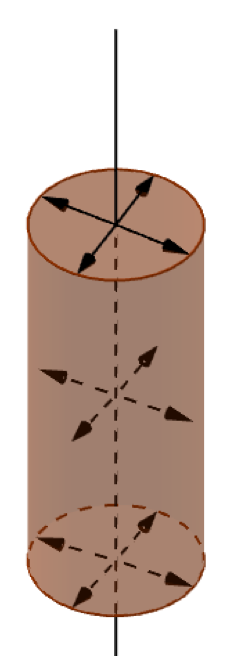
\includegraphics[height=150pt]{dlcarica}\\
	\textbf{Esempio grafico :} scelta della superficie
\end{center}
    
\pagebreak
In tale figura il contributo del campo elettrico al flusso \`e nullo per le basi del cilindro (dove le linee di campo sono parallele), mentre \`e massimo per la sua superficie laterale (in quanto ogni suo punto \`e normale alla linea di campo elettrico). Pertanto si ha che:
$$ S = S_{laterale} = 2 \pi r h $$
$$ \sum{Q_{interne}} = h\lambda $$
$$ \Phi_S\left(\vec{E}\right) = \frac{\sum{Q_{interne}}}{\varepsilon_0} = \oint_{S}{\vec{E} \cdot \hat{n}} $$
$$ \oint_{S}{\vec{E} \cdot \hat{n}} = |\vec{E}| 2\pi rh $$
$$ \frac{\cancel{h} \lambda}{\varepsilon_0} = |\vec{E}| 2\pi r \cancel{h} $$
$$ |\vec{E}| = \frac{\lambda}{2 \pi r \varepsilon_0} $$
	
$\hfill\square$